\chapter{Assessment and Conclusions}
This chapter includes an overview and assessment of the work conducted in this thesis, bringing together the ideas from the initial research and how these have helped in developing the methodologies introduced in later chapters. The validations from the methods are further assessed, followed how an explanation of how the research forming them may be taken further in potential future projects. Finally, an overview of the thesis in terms of its contributions is described.


\section{Analysis of Research and Results}
Following is an analysis of the research carried out over the stages described in the main chapters of this thesis, from the initial research into retweeting and the social graph through to the interestingness inference methodologies explained in later chapters.

\subsection{Summary \& Analysis of Initial Research}
Initial research was conducted into the act of retweeting and Twitter in general for the purposes of providing a background and foundation for the later work. In particular, research was carried out into retweet \textit{groups} and the properties and behaviours they demonstrate. During the review of the relevant literature in the field, it was indicated that a Tweet's popularity cannot generally be directly tied to the Tweet's interestingness due to factors relating to user \textit{influence}.

In the initial explorative analyses into Twitter and retweets, it was found that, agreeing with other research in the area, retweet groups, which represent the set of retweets (and their authors) of a particular Tweet, can have widely ranging sizes and depth. The path-length of a retweet group's branch was defined as the number of retweet hops between the author of the initial Tweet and that of the final retweet of the chain. This phenomenon takes into account that retweets can, themselves, be retweeted, and that retweet groups do \textit{not} consider the followships between the set of users they represent. Retweet groups were found to present an average \textit{maximum} path-length of around two, and the longest maximum path found in the dataset collected from retweets on the public timeline was of length nine. This demonstrates a significant penetration through the social graph, especially considering the `real' world's six degrees of separation, and that social networks often exhibit a social graph even more closely connected than this.

This, and other retweet group analyses, led more onto more focused research on Twitter's social graph, which began by studying the properties of the \textit{audience} size attainable through retweet groups, and the overhead generated through shared followships, and ties between users involved in retweet groups and their relationships on the social graph. It was found that the chance of a retweeter retweeting a Tweet was significantly greater to occur in cases where the retweeter follows the author of the original Tweet, but that as retweet pathways become longer, the chances of the final retweeter following the original author diminishes over the distance, demonstrating strong correlations between the edges separating users on the retweet graph and those on the social graph. These experiments were conducted using a trained logistic regression to predict a retweet outcome decision for each user who received the Tweet during simulations of each structure type.

The correlations and results from the explorative analyses on the social structure and the arrangement of users on the social graph indicated that the social structure of Twitter clearly affects the propagation of retweets and that this property could provide a useful way of estimating Tweet interestingness. This triggered research focussed on examining the differences in propagation patterns in order to demonstrate that each structure type can present very different retweet propagation patterns. Because the propagation pattern difference at this structural level was so large, it was decided that this could be a basis for an interestingness inference methodology. This method utilised the same research and algorithms behind those used in the graph structure analysis to predict a retweet count for a given Tweet within a graph of connected users, and worked through a simple comparison between this predicted value and the \textit{observed} retweet count of the Tweet. This method was not shown to perform particularly well in the validation tests conducted, and thus improvements were necessary before any further analyses were made.


\subsection{Summary of the Improved Methodology}
Improvements over the previous methodology were based around the introduction of interestingness \textit{scores}, with which Tweets could be ranked according to the ratio of their observed and expected popularities, and where if the observed popularity is proportionately larger than the expected popularity, the score for that Tweet would also be proportionately greater. This in itself provides many benefits over the previous system, which was unable to provide any indication over \textit{how} interesting a Tweet is.

The prediction of the esitmated retweet count was altered so that they could be generated directly through the use of a Bayesian network machine learning classifier, which made predictions based on a larger set of Tweet and environmental network features. These features could be collected much more efficiently from Twitter's REST API, illustrating another advantage in terms of the ease with which predictions (and thus score assignations) can be made. 

Furthermore, the efficiency stretches to providing a more universal approach, allowing Tweets from most users on Twitter to be evaluated equally and on the same scale, since the complexity of any part of the assignation process is not affected by the influence or other properties of the author user. 


\subsection{Analysis of Validation Results}
Producing the scores partially relies on the initial accuracy of making retweet predictions in the \textit{general case}, using cross-validation tests on the Bayesian network classifier and the binning policy of retweet counts explained in the prevoius chapter. The performance of each factor is highlighted in Tables \ref{table:classifierperformance} and \ref{table:binperformance} respectively, which demonstrated that a decent precision and recall could be obtained in cases using up to between 15 and 20 nominal bins. Although the binning algorithm was responsive in terms of the range and distribution of retweet counts in the set being analysed, it was aimed to achieve a projected bin count of 10 in the case of producing the global model. When generating the user-specific classifier models, the number of bins ranged significantly depending on the relative influence of each user, as described previously.

The mention of the ``general case'' is important, since the methodology is designed to discover Tweets which do \textit{not} fit this case, as these would be the Tweets which have a greater (or smaller) retweet count than expected, and would therefore be the Tweets which would contribute negatively to the aforementioned performance analyses of the prediction method. As such, if all Tweets fit their general cases as given by their features and the features of their authors, then the general performance of the cross-validations on the classifier could be greater, but then no interestingness inferences could be made.

Two main human validation tests were conducted into the performance of the scoring mechanisms provided by the improved methods; one based on interestingness decisions from non-related participants, and another based on decisions from Twitter users to whom the Tweets assessed are more relevant, as denoted by the followships of the author users. These validations expressed a good performance of the scoring scheme in a variety of ways, from the ranking of Tweets in order of interestingness through to analyses into the motivation of Tweet selection from the \textit{disparity} of Tweet scores in the timeline.


\subsection{Methodology Evaluation}
The background chapter of this thesis described other similar research in this area along with the strengths and weaknesses of each. Whilst this included a fair amount of research into retweet decision and count predictions, they are often quite similar to one another, and these goals are not the primary focus of the work in this thesis. Instead, research into information interestingness with regards to Twitter will now be evaluated against the methods outlined in this thesis.

\cite{gransee12} introduced a system for scoring Tweets based on a na{\"i}ve Bayesian classifier. The authors' learner was concerned only with textual cues for producing a score. The learner was trained using a set of Tweets from a particular author, with each Tweet being assigned a score based, similar to the work in this thesis, on the distance between the observed retweet count of the Tweet and the single \textit{baseline} retweet count for the Tweet's author at that particular time. Words in unseen Tweets are then scored individually according to the scores of Tweets the words have previously been seen in, which, when averaged, generates a score for the unseen Tweet.

The scoring method discussed in this thesis is superior to this methodology in a number of ways. Firstly, this method requires a pre-built dictionary of words to be generated and scored for each user before a model can be trained and any scores can be assigned, meaning that it is not possible to carry out on-demand assignations of scores to Tweets. Additionally, a baseline retweet count needs to be maintained for each user assessed for specific time-intervals, meaning that the scores of words in the dictionary also need to be updated periodically to reflect the change in baseline. The authors admit that their methods work better when Twitter users are more predictable and use similar words across Tweets. Finally, assessments were only made for the \textit{top} 175 users on Twitter, with no indication of its performance on users who are less influential and typically receive far fewer retweets per Tweet and users who do not Tweet enough in each time-frame for a suitable baseline value to be calculated. Influential users are generally subject to smaller fluctuations in the social graph, as additional followers wouldn't have such a large impact, and thus the retweet count baseline wouldn't vary as often as with less influential users. Therefore it would be more difficult to apply this method to Tweets from `normal' (or less influential) users.

The notion of Tweet scoring was also considered by \cite{alonso10} with a focus on determining non-interesting information, in which the authors used a scoring scheme that assigned an integer value to each Tweet of between 0 and 5. Howevever, their results are largely simply based on assigning a Tweet as interesting \textit{if it contains a URL}, which, again, does not allow the method to be appropriately applied to a wider range of Tweets. Crowdsourcing is used as part of obtaining human input for determining interestingness, but the MTWs are instructed what to class as interesting instead of allowing participants more reign on what constitutes the \textit{most} interesting. Generally, these features are not comparable to those in the methods discussed in this thesis, since the authors are more concerned with finding \textit{un}interesting Tweets to be disregarded from a stream, have a limited scoring range and do not conduct as rigorous validations into their results. Despite achieving some accurate results, the methods cannot be used on such a wide variety of Tweets as is available on Twitter.

Finally, \cite{lauw10} presented a study that used a clustering algorithm to estimate a Tweet's \textit{quality} based on a function of a Tweet's audience size and its relation to other similar Tweets. The authors' research is based around news stories, in that Tweets `belonging' to the same event are clustered together and are assigned a quality depending on the size and `importance' of the cluster. Despite the similarities in terms of assigning a quality to clusters and Tweets, the authors do not take into consideration many of the factors discussed in this thesis (including the notion of timeline `slip' discussed in chapter 4, which is relevant to their work) and the verifications conducted into the performance of their methods are not rigorous enough to prove that the quality level assigned to each cluster or Tweet is accurate or appropriate.


\section{Further and Future Work}
There are various ways in which the work and research in this thesis could be taken further in extended work and projects.


\subsection{For marketing purposes}
As part of the procedure for assigning scores to a Tweet, it was necessary to produce an \textit{expected} retweet count for it. This is a prediction based on the Tweet's user and author features and the similarities of these to previously-seen Tweets. Although the interestingness inferences are based on the expected count being different from the actual retweet count, it was shown that the classifier and binning algorithms used demonstrated a good performance in classifying the retweet outcome for a given Tweet. 

As such, it is sensible to assume that this predictor could be taken further in assisting Twitter users in constructing Tweets which are likely to attract more retweets. Before posting a Tweet, a system could use a trained classifier to indicate how many retweets the Tweet is likely to receive. With respect to the interestingness scores produced by the full methodology, these could be useful for retrospectively returning feedback to users in order to highlight the Tweets that were more popular than expected and to perhaps illustrate any common features found in Tweets that were more popular than those that weren't. 

Of course, isolating the notion of popularity from the static features of a Tweet in the general case forms part of the motivation for this research, but the value of features for some users may have more of an effect on their retweet receipts than on other users. For example, a Twitter account representing a news service is more likely to receive retweets of Tweets that contain a URL than an account representing a parody celebrity account, who is likely to obtain retweets more through the wording and relevance of the content of the actual Tweet.


\subsection{Building on the social structure}
Chapter 4 of this thesis included research into the social structure of Twitter and the role this played in the retweet propagation patterns of the information flow within it. The impact of the structural changes on the propagation pattern led the way in building the initial interestingness inference methodology, which was based on simulating Tweets and retweet decisions through social structures reflected directly from Twitter.

The method had many drawbacks, as described earlier, but mainly these were due to its inefficency in terms of the amount of data necessary in order to construct the local networks, which included all the users and edges within two hops of the source author user. Two hops was chosen, as three or more was prohibitively complex to collect and implement, and since two was found to be the average \textit{maximum} path-length of Tweets analysed in chapter 3. Despite this, the limitations in data collection meant that Tweets could only realistically be simulated for users with much smaller local networks, and thus the methods could not be applied to a wide variety of Tweets on Twitter or have inferences made on demand.

The research in this thesis then followed a different path in an attempt to solve the presented problems, but there are ways in which the previous method could be improved more directly. One way, in particular, would be to attempt to \textit{infer} or `estimate' a user's local network from a set of its immediately-available parameters. Analytical results from this first methodology highlighted correlations between a user's follower count and the size of the user's local follower network, and a correlation between the size of this local network and the edge density of the users within it, as illustrated by Figures \ref{fig:network-followers} and \ref{fig:network-density}.

\begin{figure}[h]
\begin{subfigure}{.5\textwidth}
    \centering
    \begin{tikzpicture}[scale=0.8]
    \begin{loglogaxis}[
            ylabel=$\foc{\aut{t}{O}}$,
            xlabel=$n$,
            grid=major,
            xmin=1E4,
            xmax=1E6
                       ]
       \addplot[mark=+,only marks,blue] plot coordinates{
            (15244,28)(20273,38)(26943,56)(28279,41)(39192,56)(58650,80)(67585,125)(90366,170)(109982,230)(112070,135)(118854,279)(132497,273)(184158,291)(258252,388)(352661,617)(368389,628)(561100,928)(666690,900)        
        };    
    \end{loglogaxis}
    \end{tikzpicture}
    \caption{Relationship between local network size ($n$) and the follower count of an author of Tweet $t$.}
    \label{fig:network-followers}
\end{subfigure}
\quad
\begin{subfigure}{.5\textwidth}
    \centering
    \begin{tikzpicture}[scale=0.8]
    \begin{loglogaxis}[
            ylabel=$d$,
            xlabel=$n$,
            grid=major,
            xmin=1E4,
            xmax=1E6
            ]
       \addplot[mark=+,only marks,blue] plot coordinates{
            (352661,4.49E-06)(37084,3.20E-05)(10631,0.000103613)(184158,6.97E-06)(39192,2.74E-05)(90366,1.62E-05)(33520,4.00E-05)(72123,1.71E-05)(112070,9.40E-06)(72069,1.70E-05)(132497,9.19E-06)(368389,4.06E-06)(358200,5.29E-06)(118854,1.10E-05)(109982,1.10E-05)(15244,7.50E-05)(382357,3.39E-06)(15273,7.03E-05)(106877,1.03E-05)(28279,3.72E-05)(18366,5.84E-05)(666690,2.40E-06)(205417,5.21E-06)(26943,3.87E-05)(19385,6.16E-05)(561100,2.61E-06)(58650,1.75E-05)(258252,5.11E-06)(106247,1.04E-05)(32300,3.22E-05)(67585,1.63E-05)
        };    
    \end{loglogaxis}
    \end{tikzpicture}
    \caption{Relationship between local network size ($n$) and local graph edge density ($d$).}
    \label{fig:network-density}
\end{subfigure}
\caption{Plots illustrating indirect correlations between an author user's follower count and the edge density of the author's local network}
\end{figure}

A graph's edge density can be calculated as a function of the number of nodes and edges existing within the graph;
\[
    d = \frac{|E|}{|N|(|N| - 1)}
\]

This suggests that a user's follower count could be used to indirectly estimate the edge density of that user's local follower graph. Since Figure \ref{fig:real-scalefree} showed the similarities, along with other research covered in the Background chapter, between the structure of Twitter's social graph and that of a similarly-sized scale-free network, it is indicative that a faux scale-free network could be generated with a provided edge density and size in such a way as to reflect the user's own local network. Although this would not be an intricate mapping of the users and edges existant in reality, it would provide an appropriate size and density of edges between the nodes, within which Tweets could be propagated and examined.

Through generating a graph structure in this fashion, then there is no need to collect the local network information for each user to be assessed, since a faux graph could simply be created on the fly, and Tweets from more influential users could also be simulated (depending on the computational complexity of the generation algorithm and simulator). The \textit{accuracy} of the interestingness inference could then be improved through a larger training set, the use of more features for handling the decisions, or by introducing further routines to make the simulations and the decisions more realistic. 


\subsection{Taking the scoring methodology further}
There are various ways in which research could be carried out into the methodologies behind the scoring mechanism used in the interestingness inferrer discussed in chapter 5. In particular, one could be to research into `unnecessary' edges between users in OSNs. The final validations conducted on this method involved participants assessing the Tweets they'd naturally receive onto their home timeline as they are from users that they already \textit{follow}. 

However, as has been made clear at points in this thesis, not \textit{all} the information a friend posts is likely to be interesting, and that particularly interesting information from a particular source is likely to be retweeted more than less interesting information posted by the same source. If a particular destination user finds only a small subset of Tweets from a source to be interesting, and that these Tweets are therefore more likely to be retweeted by other users also following the source, then is there a non-direct pathway available between the source and the destination user that the interesting Tweets could be passed down?

\begin{figure}[h]
\centering
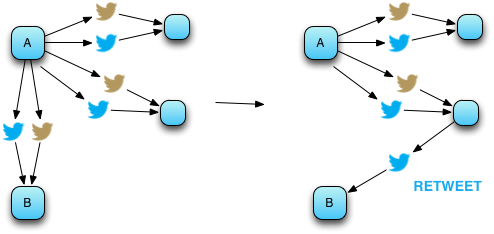
\includegraphics[scale=0.8]{6.Conclusions/Media/retweet_path.png} 
\caption{Removing an `unnecessary' link between users on the social graph.}
\label{fig:removed_link}
\end{figure}

If this is the case, as with Figure \ref{fig:removed_link}, then the link representing the followship between the destination user (B) and the source user (A) could be unnecessary, since user B is receiving a fair amount of noise from user A, but the interesting information produced by user A could still reach B through retweets carried out by other followers of A. 

Whilst a lot of this is hypothetical, it would provide an interesting extension to the research carried out in this thesis, in that interestingness scores could be used to assign thresholds of interestingness to users with the aim of discovering whether interesting Tweets could still be propagated to the extent that they deserve, yet by simultaneously reducing the propagation of noisy information. 

Since it has been explained how a user's followships act as a `search term' for information retrieval on Twitter, by finding ways of forwading interesting information to users who do not directly follow a source, then it is clear how this could pave a way for enabling interesting and \textit{relevant} information can be delivered to users, yet without them having to look for it or know about its existence in the first place.


\section{Conclusions \& Contributions}
The final part of this concluding chapter summarises the research and processes conducted in this thesis along with the contributions made by the research it contains.


\subsection{Final remarks}
The work in this thesis was carried out with the aim of researching a methodology that is able to suitably infer interesting information in Twitter. Although the research has focused on Twitter as a platform for information dissemination, the motivation for this research stems from the \textit{noise} observed every day in all online social networks that support information propagation, including those such as Facebook and Tumblr.

The research processes culminated in the development of a method that ranks Tweets by assigning a score indicating an estimated level of interestingness based on a function of its perceived popularity. The methods were verified through the use of crowd-sourced validation tests covering the notions of general interestingness (in terms of identifying it from `noisy' information) and of more \textit{relevant} interestingness (through assessments of Tweets authored by more relevant users).

Analyses into the validation tests demonstrated the process by which users are able to identify interesting information and showed that the scoring mechanism is able to effectively rank Tweets in an appropriate order of interestingness in both mixed timelines and in timelines of Tweets authored by the same user. The scores can be applied to Tweets from all users on the same scale, meaning that inferences are not limited to a specific subset or type of Tweet.

The methods are open enough and use resources that are mostly common to many similar social networks. For example, ``shares'' and ``reblogs'' can be examined as the propagation mechanisms in Facebook and Tumblr, respectively, in attempts to apply the same scoring schemes to other platforms.


\subsection{Contributions}
The research in this thesis makes several contributions to social media analytical research. The main contributions are outlined below.

A comprehensive survey is carried out into relevant literature in information propagation in online social networks, along with evaluations and assessments of some of the research more specific to inferring interestingness.

Retweet properties and the way they are influenced by the social graph are thoroughly researched in order to provide a general background and understanding of the notions relating to propagation in online social networks, propagation and information penetration, Tweet `audience', and how these factors are related to the arrangement of users on the social graph. The definition of terms, such as `retweet group' and `maximum path-length' are useful for discussing various properties relating to retweeting on Twitter.

An investigative study is made into the use of machine learning techniques and classifiers in the field of social media, and the ways in which they can be useful for different purposes.

Finally, a method for suitably predicting estimated retweet counts, as dynamically nominal categories, is described, implemented and verified, leading to the development of a method for assigning interestingness scores to Tweets as part of an effort to support the ranking of Tweets and of higlighting interesting Tweets from the noise of everyday communication on Twitter.
